\section{Experimental validation}\label{sec:experiments}

\todo[inline]{WIP}

In this section, we aim to validate the utility of the CLEAVE framework through a series of experiments.

\todo[inline]{talk about goal of experiments}

We depict our experimental setup in \cref{fig:cleave:expsetup}, consisting of a single control loop deployed across a pair of consumer-grade computing devices.
We employ a Raspberry Pi 4B single-board computer together with a general-purpose \verb|x86_64|-based workstation.
These devices are connected to each other by an 802.11n WiFi link.
For ease of deployment and reparametrization, we deploy our CLEAVE control loop as a pair of Docker~\cite{merkel2014docker} containers\todo{add link to image?}; one for the plant, running on the Rasberry Pi device, and one for the Controller, running on the workstation. 
These instances are then connected to an overlay network configured through Docker which sits on top of and abstracts away the real network configuration, and allows for transparent communication between the Plant and Controller.

\begin{figure}
    \centering
    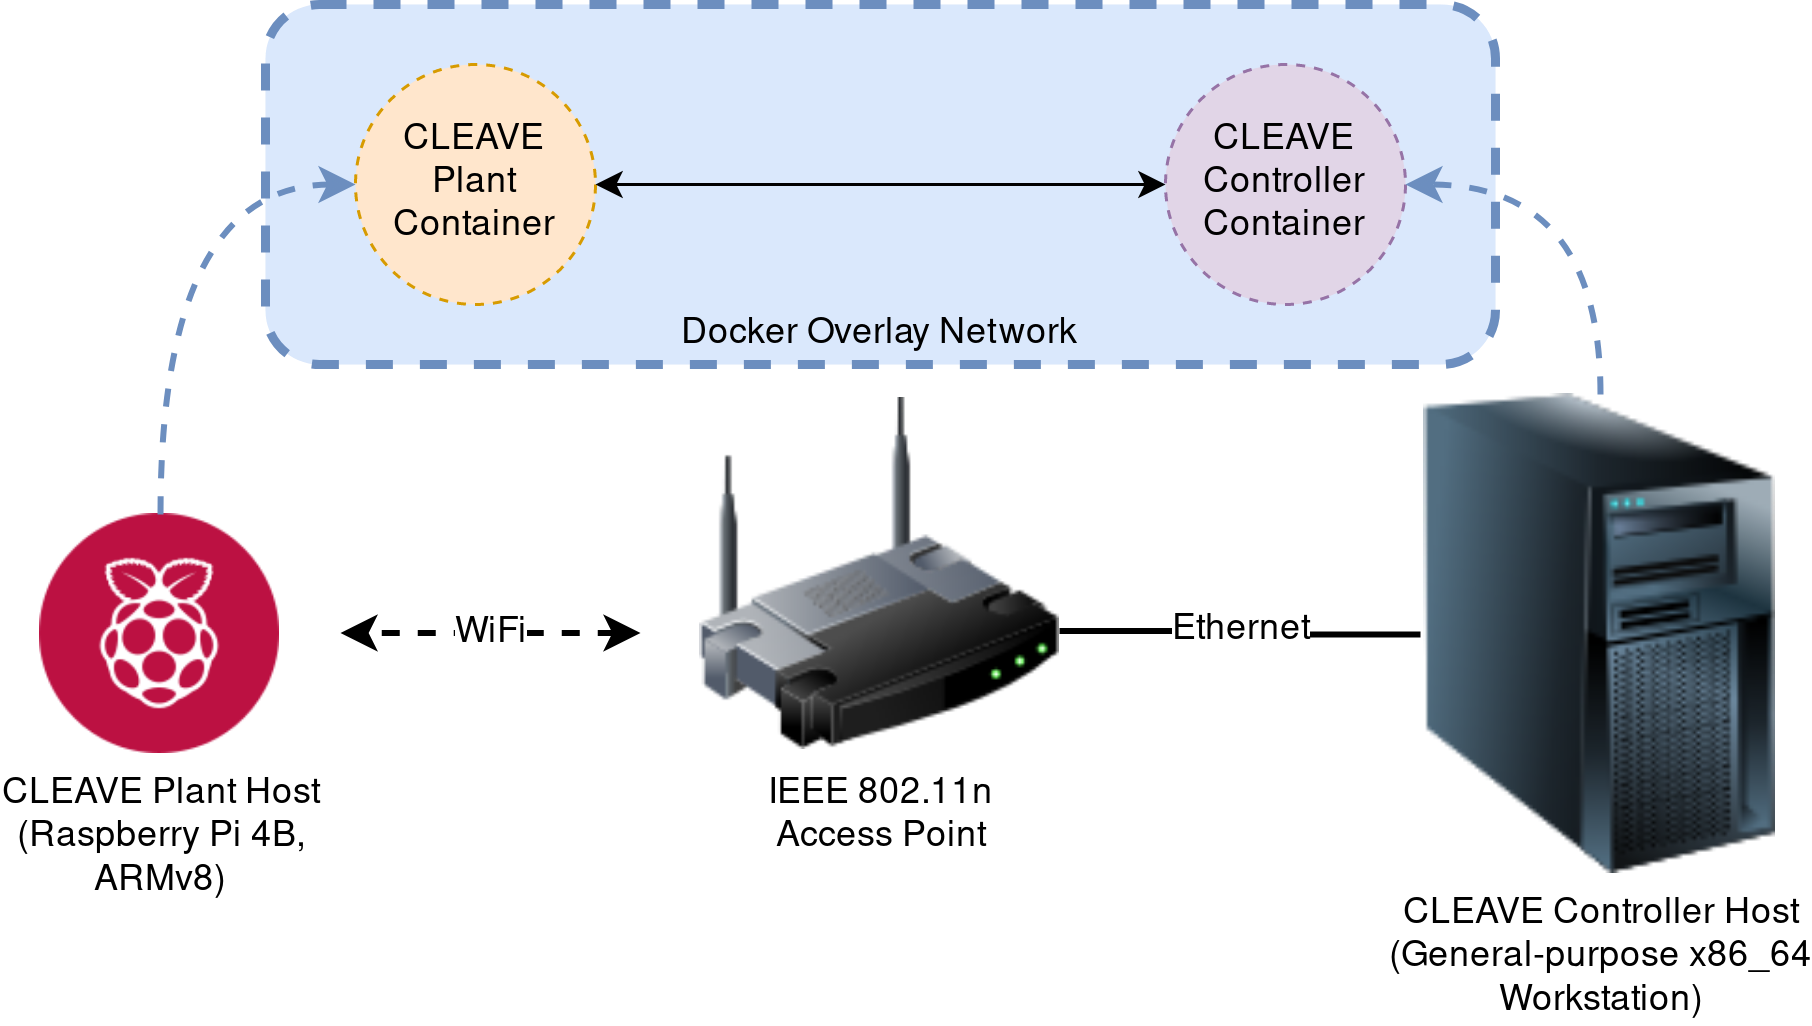
\includegraphics[width=.95\columnwidth]{images/CLEAVE_experiment_setup}
    \caption{Experimental setup. Containerized versions of the core CLEAVE emulation components are deployed inside a Docker Overlay Network spanning a Raspberry Pi 4B Plant host connected to an x86 Controller host over a 802.11n WiFi link.}\label{fig:cleave:expsetup}
\end{figure}

We use a two-dimensional inverted pendulum system for the control system deployed inside CLEAVE for the experiments, 
This system was chosen due to its relative simplicity and prevalence in the field of automatic control as one of the fundamental examples of linear control.
The physical system, represented in \cref{fig:invpend}, is implemented using CLEAVE's API and a 2D physics library~\autocite{chipmunk2d,pymunk}.
For the controller, a proportional-differential strategy is employed, implemented using the framework Controller API and the NumPy numeric computation library~\autocite{harris2020array}.

This setup is then used to run a series of experiments with varying parametrization of the controlled system.
Specifically, we modify:
\begin{itemize}
    \item the sampling rate of the Plant state, setting it to \SIlist[list-units=single,list-final-separator={, or }]{5;10;20;40;60;120}{\hertz};
    \item the responsiveness of the Controller, by adding fixed delays of  \SIlist[list-units=single,list-final-separator={, or }]{0;25;50;100;200}{\milli\second} after the processing of each sample.
\end{itemize}
Each one of the \num{30} possible combinations of these parameters is run on the experimental testbed depicted in \cref{fig:cleave:expsetup} for \num{10} repetitions lasting \SI{5}{\minute} each, yielding \SI{25}{\hour} worth of data.
During each repetition, we collect detailed data on both the state of the controlled system as well as on the data sent over the network.


\begin{figure}
    \centering
    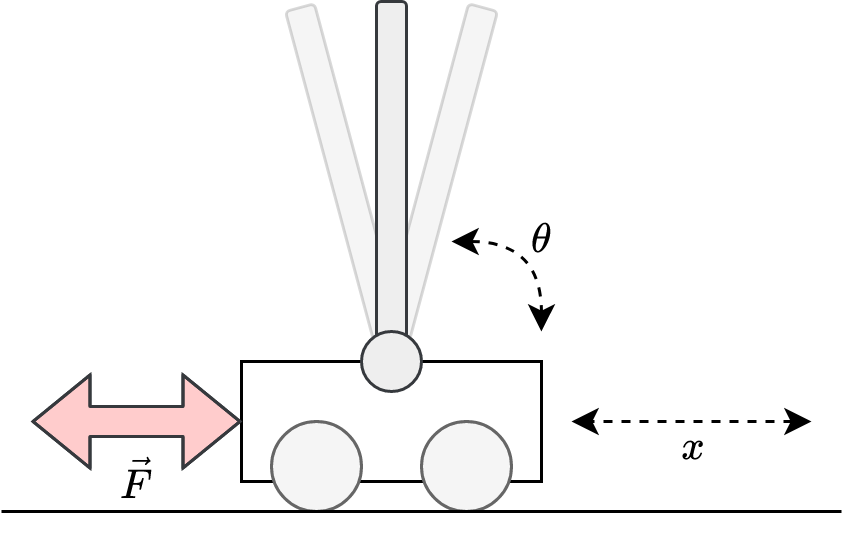
\includegraphics[width=.95\columnwidth]{images/inverted_pendulum.png}
    \caption{
        The two-dimensional inverted pendulum system.
        The cart moves on the X-axis, and the pendulum on top of it swings freely.
        The objective of the system is to balance the pendulum vertically through the application of horizontal forces on the cart.
    }\label{fig:invpend}
\end{figure}